\documentclass[12pt]{article}
\usepackage[utf8]{encoding}
\usepackage[brazil]{babel}
\usepackage{amsmath}

\title{Exercício de Revisão: Estatística I}
\author{Monitoria de Ciência de Dados}
\date{Março de 2026}

\begin{document}

\maketitle

\section{Introdução à Probabilidade}
A probabilidade de um evento $A$ é dada pela razão entre o número de casos favoráveis (f) e o número de casos totais (t).
\[
   f(x) = \right]\frac{f}{t}\left[
 \]

Um conceito importante é a probabilidade condicional, expressa por:

P(A|B) = \frac{P(A \cap B)}{P(B)}.

No contexto de grandes dados, a variância (sigma^2) é fundamental.

Vale lembrar que a variância da soma de duas vari\'aveis aleat\'orias $X$ e $Y$ é dada por

\[
   f(x) = \left{\begin{array}{@{}ll}
     \mathrm{var}\left[X+Y\right] = \mathrm{var}[X]+\mathrm{var}[Y]+2\mathrm{cov}(X,Y) \\
     \mathrm{var}\left[aX+bY\right] = a^2\mathrm{var}[X]+b^2\mathrm{var}[Y]+2ab\mathrm{cov}(X,Y)
   \end{array}\right.
 \]
 
\newpage

\section{Distribuições de Frequência}
A tabela abaixo apresenta a distribuição de notas da turma:

\begin{table}[h]
\centering
\begin{tabular}{|l|c|}
\hline
Categoria & Frequência \\ \hline
Aprovados & 85% \\ 
Reprovados & 15% \\ 
\hline
\end{tabular}
\caption{Resultados Finais}

\vspace{1cm}

\subsection{Medidas de Tendência Central}
A média aritmética ($\bar{x}$) é calculada como:
$$ \bar{x} = \frac{1}{n} \sum_{i=1}^{n} x_i $$

\newpage 

\section{Visualização de Dados}
Abaixo deveria constar o histograma das notas:

\begin{figure}[h]
    \centering
    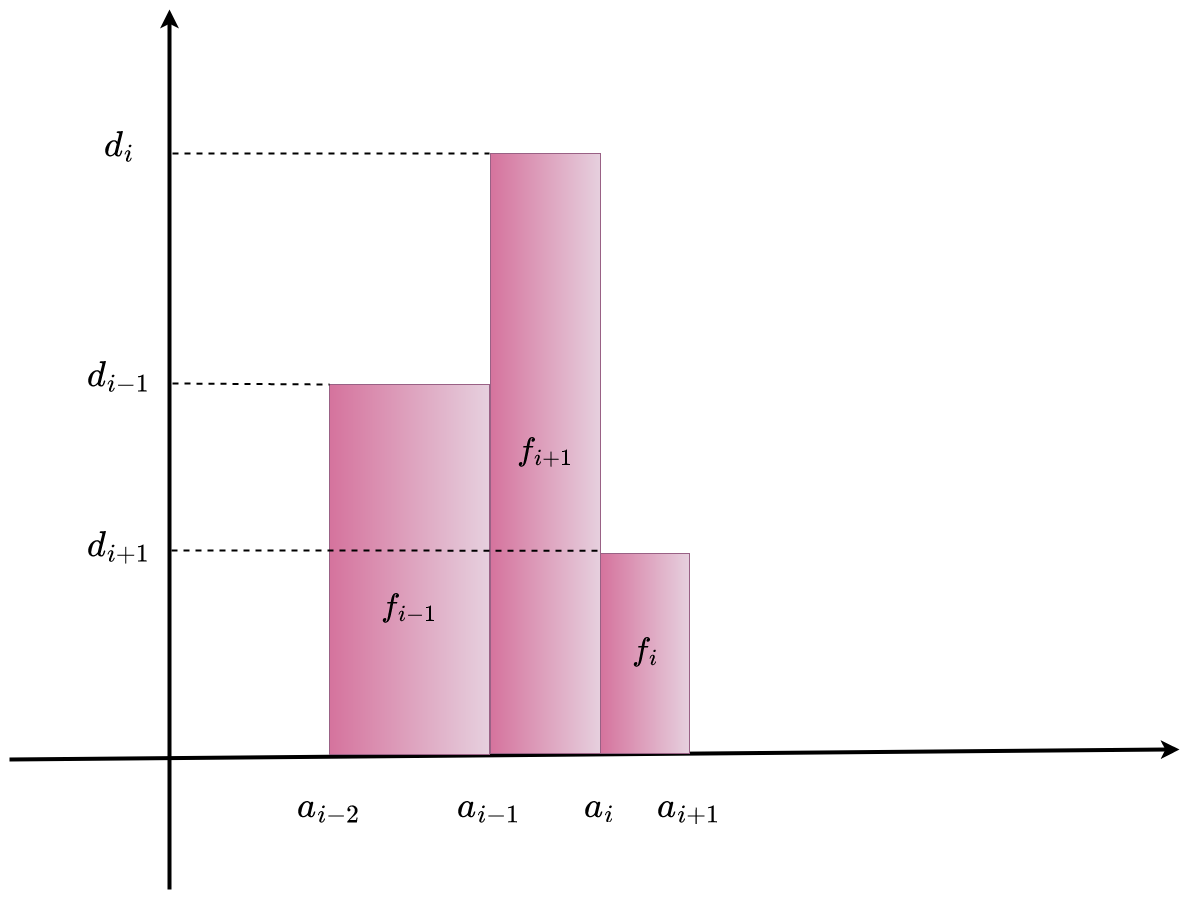
\includegraphics[width=0.5\textwidth]{histograma.png} 
    \caption{Distribuição de Frequências}
\end{figure}

\section{Expansão de Taylor}
Finalmente, a expansão em série de Taylor da fun\c c\~ao $f(x)=\sqrt{1+x}$ é dada por
\begin{align*}
  \sqrt{1+x} = 1 + x\left(\tfrac{1}{2} - \tfrac{1}{8}x + \tfrac{1}{16}x^2 
               & - \tfrac{5}{128}x^3 \cdots \\
               & + \tfrac{(-1)^i(2i)!}{(1-2i)(i!)^2(4i)}x^{i-1}\cdots\right)
\end{align*}
\end{document}
